\documentclass[12pt,a4paper]{article}
\usepackage{amsmath}
\usepackage{amsfonts}
\usepackage{amssymb}
\usepackage{makeidx}
\usepackage{graphicx}
\usepackage{enumerate}
\usepackage{setspace}
\usepackage{longtable}
\usepackage{float}
\usepackage{hyperref}
\usepackage[framed,numbered,autolinebreaks,useliterate]{mcode}

\usepackage[left=2cm,right=2cm,top=1.75cm,bottom=1.75cm]{geometry}
\author{N Sowmya Manojna}

\usepackage{fontspec}
\setmainfont{Cambria}

\usepackage{caption}
\DeclareCaptionLabelSeparator{pipe}{ $|$ }% or $\vert$
\captionsetup{font=small, labelfont={bf, color=blue}}
% \captionsetup{font=small, labelfont={bf}}

\newcommand{\spa}{\vspace{1.5em}}
\newcommand{\noi}{\noindent}
\def\dul#1{\underline{\underline{#1}}}
\def\tt#1{\texttt{#1}}


\begin{document}
\begin{titlepage}
	\begin{center}
		\vspace{3em}
		\large {BT6270 Computational Neuroscience}
		\vspace{10em}

		\rule{0.9\linewidth}{0.5mm} \\[0.4cm]
	    \large{\bfseries{Computational Neuroscience Assignment 3}} \\
	    \rule{0.9\linewidth}{0.5mm} \\[3 em]

	    N Sowmya Manojna | BE17B007\\
		Department of Biotechnology,\\
		Indian Institute of Technology, Madras\\

		\vspace{5em}
		
\includegraphics[scale = 0.09]{images/iitmlogo.png}

	\end{center}
\end{titlepage}

\section{Question 1}
\subsection{Visualization}
The images were read and converted into \tt{numpy arrays} using the \tt{numpy.loadtxt} function. In order to ensure that black pixels were represented as \tt{+1} and white pixels were represented as \tt{-1}, the sign of the array was taken. Further, the positions where the pixel value was \tt{0} was assigned to \tt{1}. The final assignment ensured monotonic error decrease.\\

\noi
The visualized images are as follows:
\begin{figure}[H]
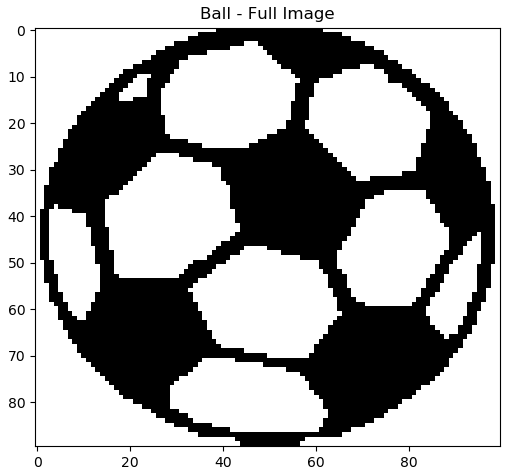
\includegraphics[scale=0.3]{images/ball.png}
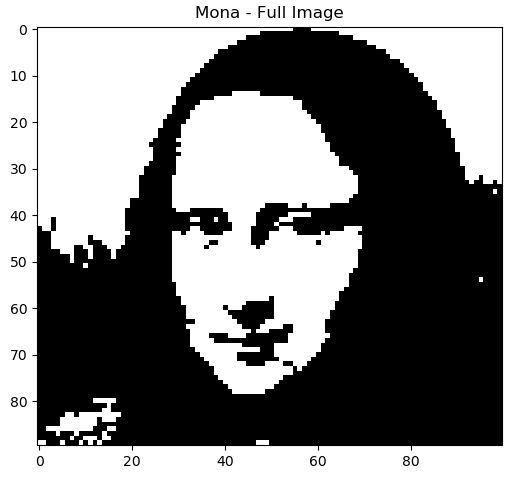
\includegraphics[scale=0.3]{images/mona.png}
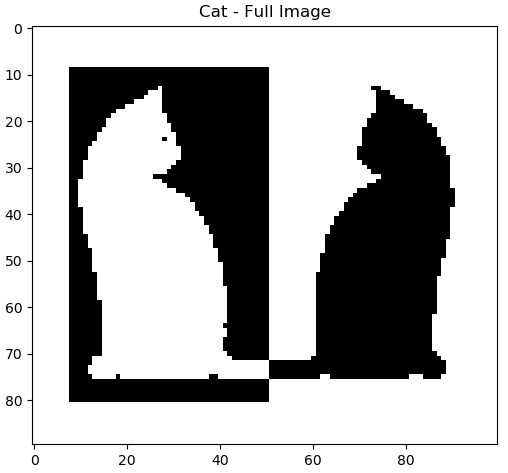
\includegraphics[scale=0.3]{images/cat.png}
\caption{Visualization of the images provided - Ball, Mona and Cat.}
\end{figure}

\subsection{Hopfield Network}
Both continuous and discrete hopfield networks were constructed. But as the discrete hopfield networks converged instantly, continuous hopfield networks were used.\\

\noi
The matrix equations used for discrete hopfield networks are as follows:
\begin{equation}
W = \frac{1}{N}SS^T
\end{equation}
\begin{equation}
V(t+1) = \sigma(WV(t))
\end{equation}

\noi
The matrix equations used for continuous hopfield networks are as follows:
\begin{equation}
W = \frac{1}{N}SS^T
\end{equation}
\begin{equation}
\frac{dU}{dt} = -U + WV
\end{equation}
\begin{equation}
V = \tanh(\lambda U)
\end{equation}

\noi
The discrete hopfield network is implemented using the function \tt{discrete\_hopfield} and the continuous hopfield network is implemented using the function \tt{continuous\_hopfield} inside the file \tt{hopfield.py}\\

\noi
The parameters - $\lambda$ and $dt$ used is $20$ and $0.01$ respectively.

\break
\section{Question 2}
\subsection{Patch Generation}
Patches with a minimum width of 20 pixels, maximum width of 45 pixels, minimum height of 15 pixels and maximum height of 45 pixels are generated at random positions of the image.\\

\noi
The patches are generated using the function \tt{get\_patches} in the file \tt{hopfield.py}


\subsection{Plot of Input Patch}
The patch generated is as follows:
\begin{figure}[H]
\centering
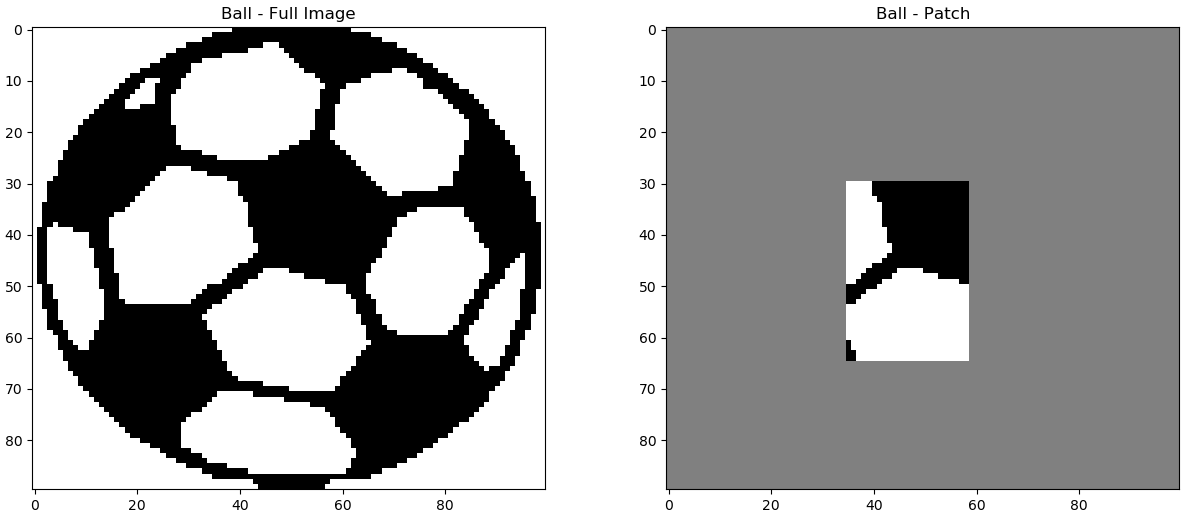
\includegraphics[scale=0.4]{images/ball_patch.png}
\caption{Patch generated as inputs to the network. The image on the left was used as the input trigger.}
\end{figure}

\subsection{Variation of RMSE across Iterations}
The variation of RMSE across iterations is as follows:
\begin{figure}[H]
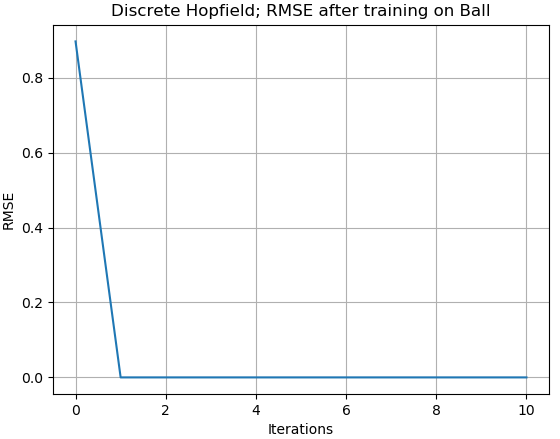
\includegraphics[scale=0.45]{images/dhn_ball.png}
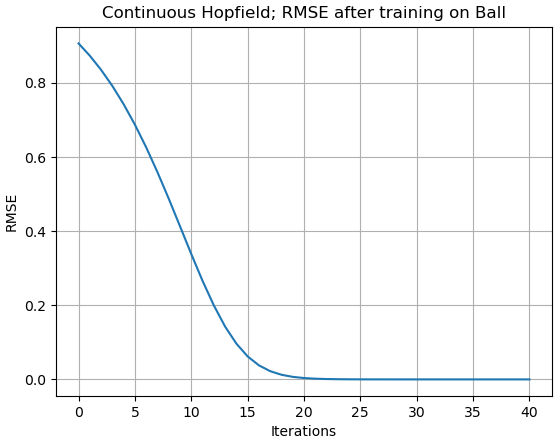
\includegraphics[scale=0.45]{images/chn_0_ball.png}
\caption{RMSE variation when trained using a (A) Discrete (B) Continuous Hopfield Network}
\end{figure}

\break
\section{Question 3}
\subsection{Plot of Input Patches}
The patches generated are as follows:
\begin{figure}[H]
\centering
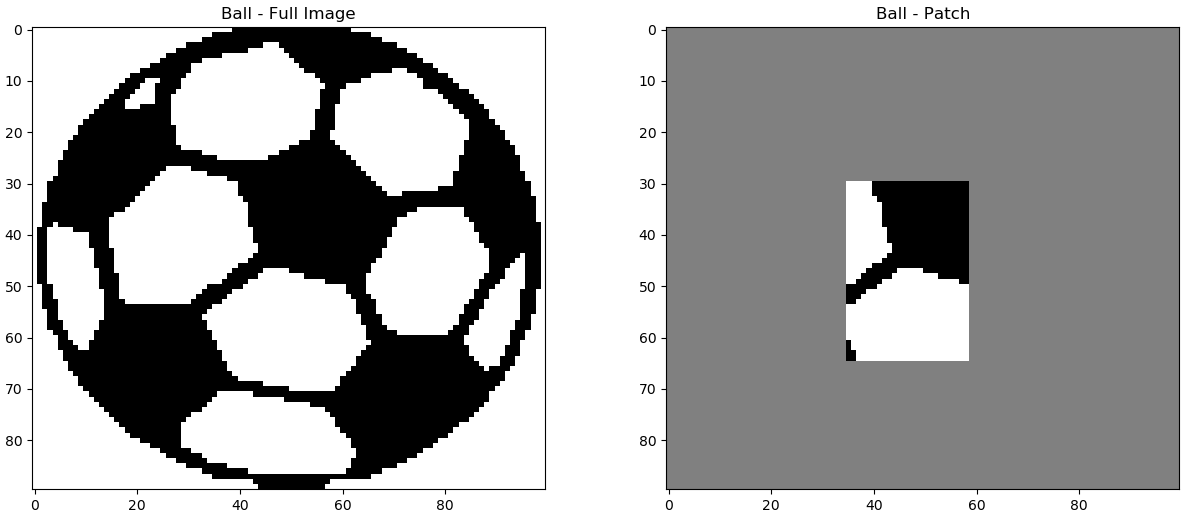
\includegraphics[scale=0.4]{images/ball_patch.png}
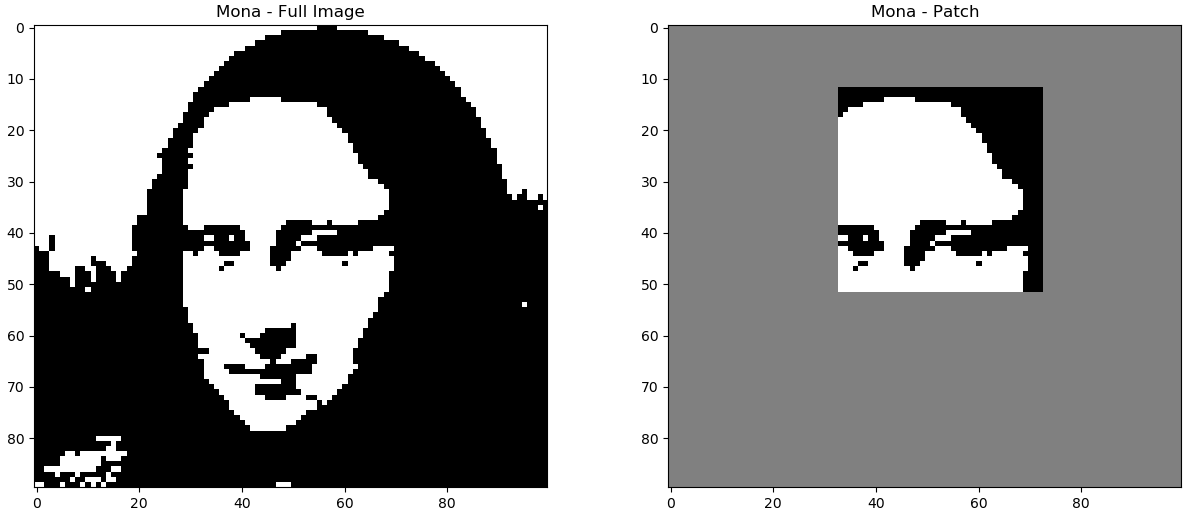
\includegraphics[scale=0.4]{images/mona_patch.png}
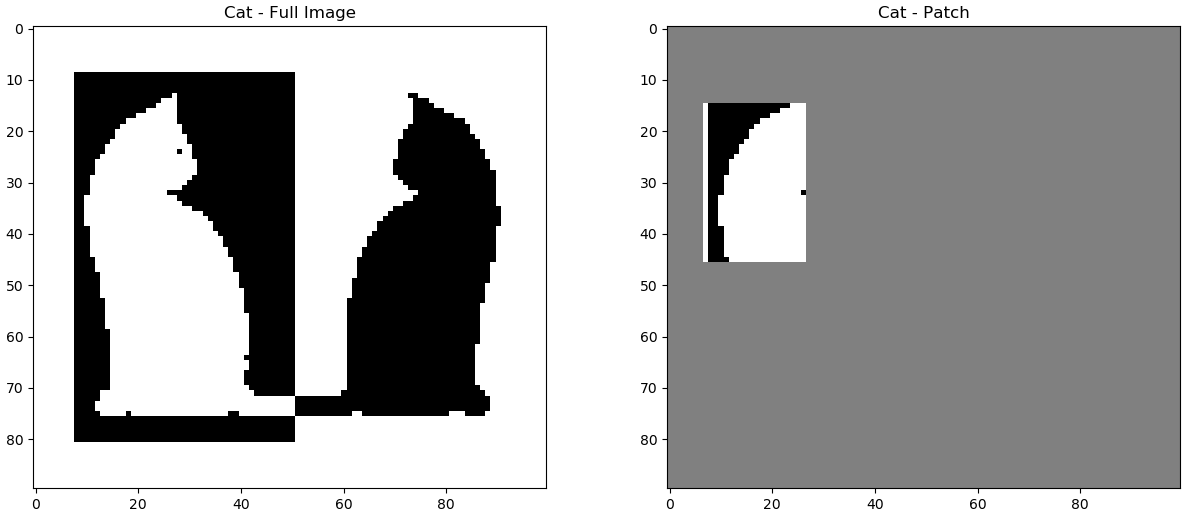
\includegraphics[scale=0.4]{images/cat_patch.png}
\caption{Patches generated as inputs to the network. The images on the left were used as input triggers.}
\end{figure}

\break
\subsection{Variation of RMSE across Iterations}
\subsubsection{Discrete Hopfield Network}
The variation of RMSE across iterations using a discrete hopfield network is as follows:
\begin{figure}[H]
\centering
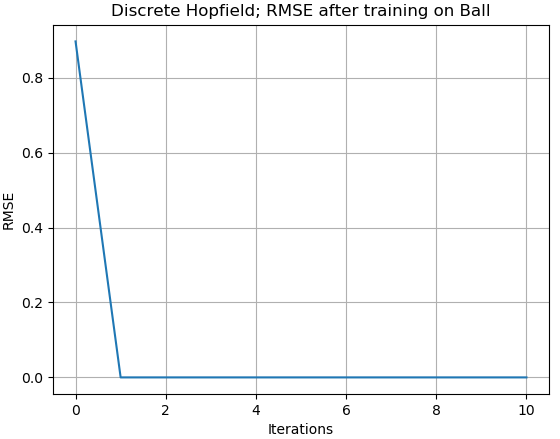
\includegraphics[scale=0.45]{images/dhn_ball.png}
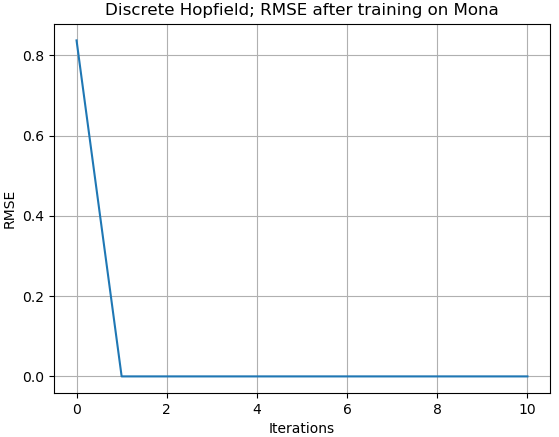
\includegraphics[scale=0.45]{images/dhn_mona.png}
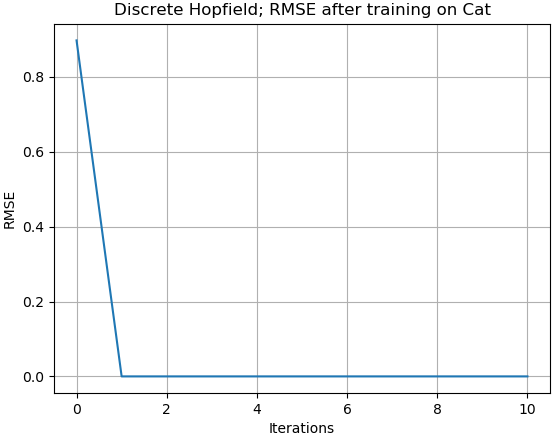
\includegraphics[scale=0.45]{images/dhn_cat.png}
\caption{RMSE variation when trained using a Discrete Hopfield Network}
\end{figure}

\break
\subsubsection{Continuous Hopfield Network}
The variation of RMSE across iterations using a continuous hopfield network is as follows:
\begin{figure}[H]
\centering
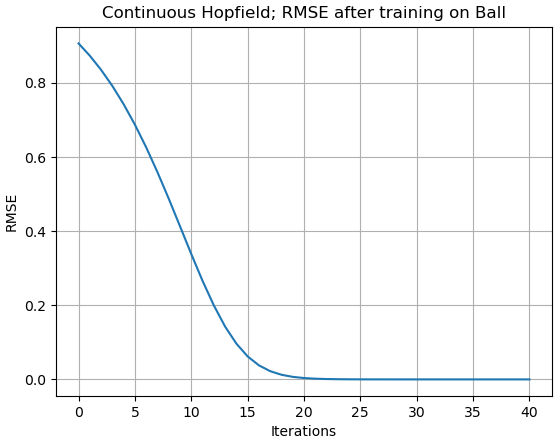
\includegraphics[scale=0.45]{images/chn_0_ball.png}
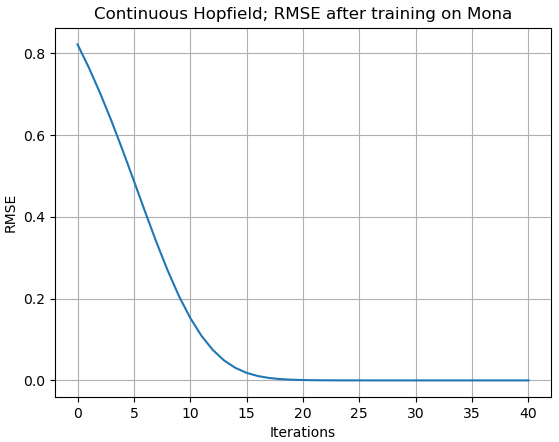
\includegraphics[scale=0.45]{images/chn_0_mona.png}
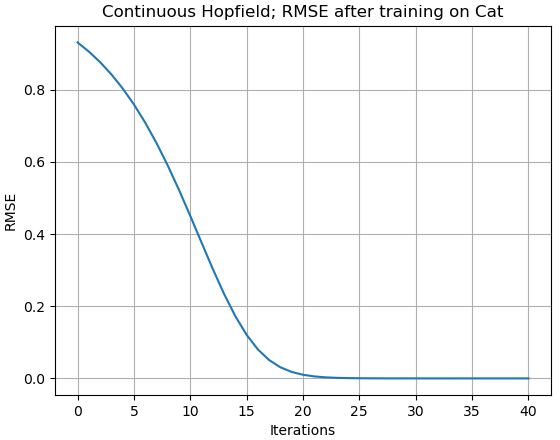
\includegraphics[scale=0.45]{images/chn_0_cat.png}
\caption{RMSE variation when trained using a Continuous Hopfield Network}
\end{figure}

\noi
Due to the smooth nature of the RMSE plots in Continuous Hopfield Networks, only they were evaluated for image retrieval after weight damage.

\subsection{Weight Damage}
\subsubsection{25\% Weight damage}
\textbf{Variation of RMSE across Iterations}\\
The variation of RMSE across iterations using a continuous hopfield network is as follows:
\begin{figure}[H]
\centering
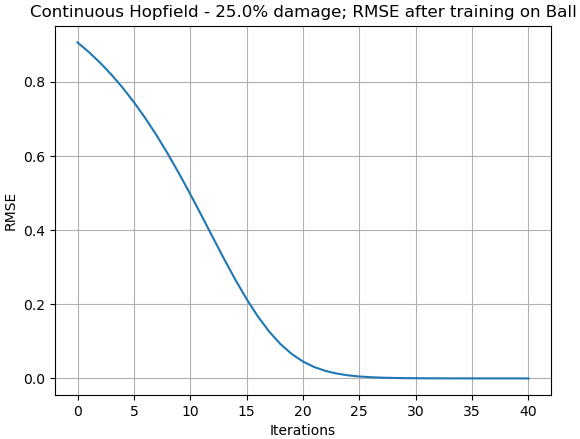
\includegraphics[scale=0.4]{images/chn_25_ball.png}
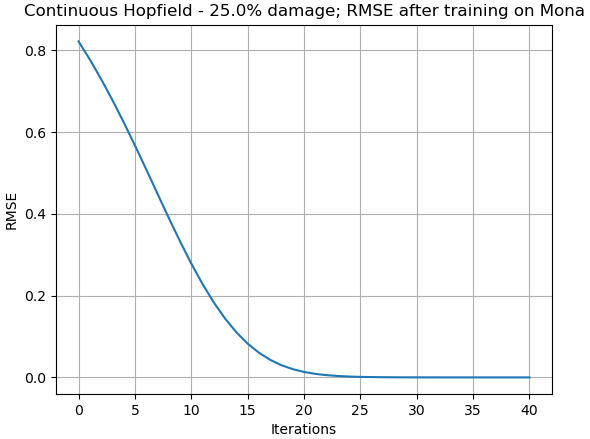
\includegraphics[scale=0.4]{images/chn_25_mona.png}
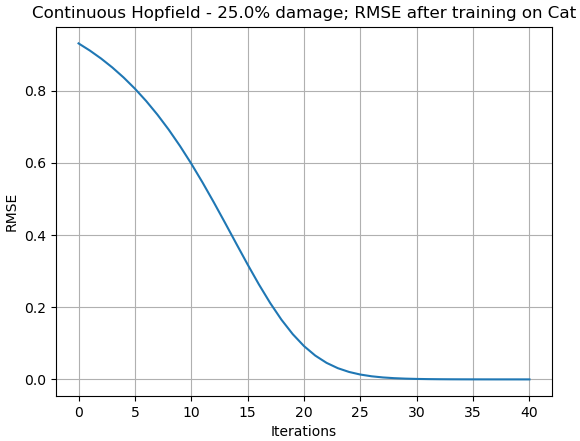
\includegraphics[scale=0.4]{images/chn_25_cat.png}
\caption{RMSE variation when trained using a Continuous Hopfield Network, with 25\% Weight Damage}
\end{figure}

\noi
\textbf{Final Image Reconstruction}\\
The final images reconstructed using continuous hopfield networks is as follows:
\begin{figure}[H]
\centering
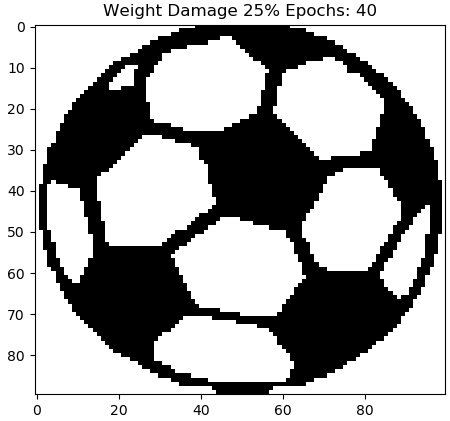
\includegraphics[scale=0.34]{images/ball_chn_25_end.png}
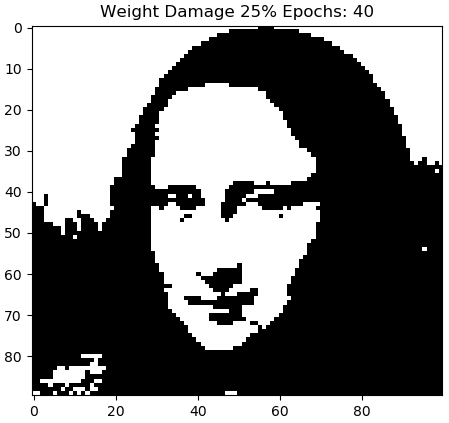
\includegraphics[scale=0.34]{images/mona_chn_25_end.png}
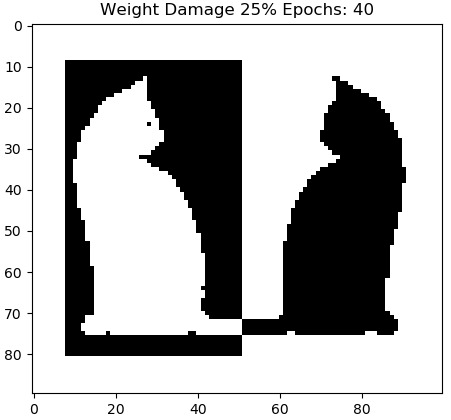
\includegraphics[scale=0.34]{images/cat_chn_25_end.png}
\caption{RMSE variation when trained using a Continuous Hopfield Network, with 25\% Weight Damage}
\end{figure}

\noi
\textbf{Image Retrieval Video}\\
The video of the image retrieval can be accessed in the files folder and are named: \tt{ball\_chn\_25.mp4}, \tt{mona\_chn\_25.mp4} and \tt{cat\_chn\_25.mp4}.


\subsubsection{50\% Weight damage}
\textbf{Variation of RMSE across Iterations}\\
The variation of RMSE across iterations using a continuous hopfield network is as follows:
\begin{figure}[H]
\centering
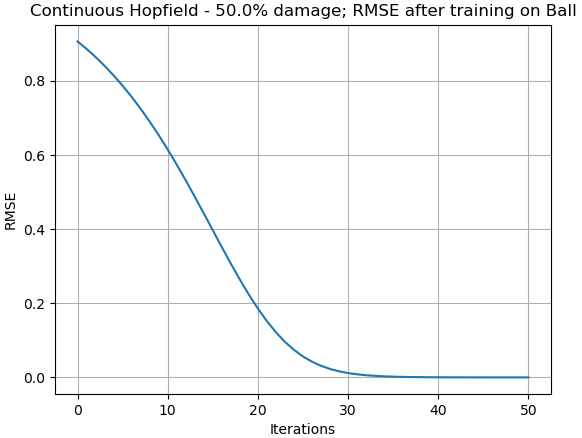
\includegraphics[scale=0.4]{images/chn_50_ball.png}
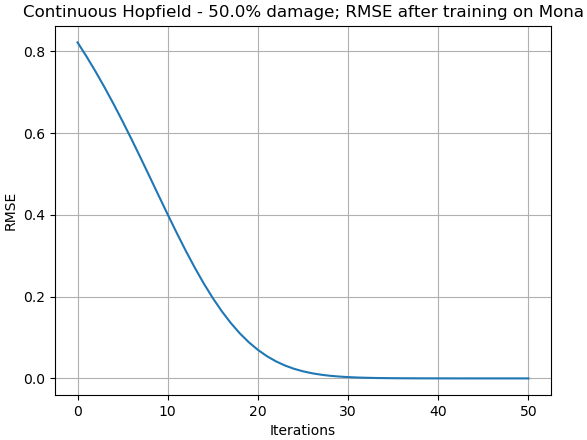
\includegraphics[scale=0.4]{images/chn_50_mona.png}
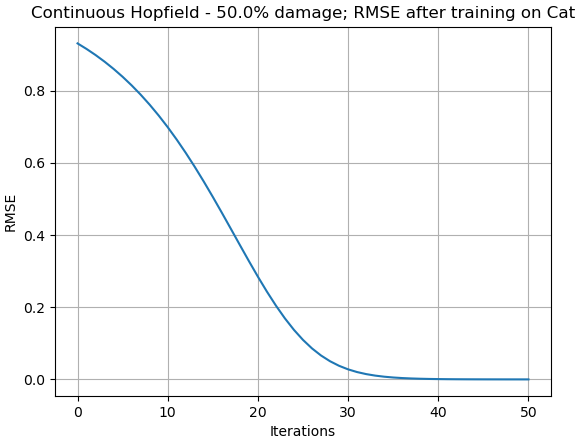
\includegraphics[scale=0.4]{images/chn_50_cat.png}
\caption{RMSE variation when trained using a Continuous Hopfield Network, with 50\% Weight Damage}
\end{figure}

\noi
\textbf{Final Image Reconstruction}\\
The final images reconstructed using continuous hopfield networks is as follows:
\begin{figure}[H]
\centering
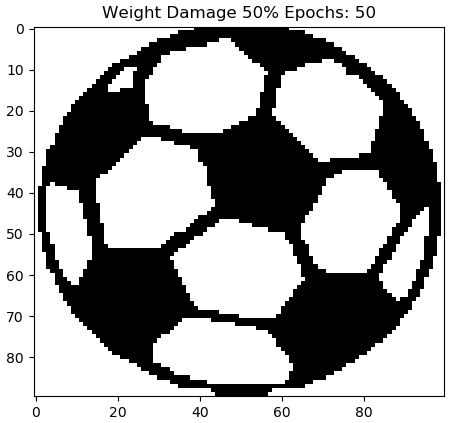
\includegraphics[scale=0.34]{images/ball_chn_50_end.png}
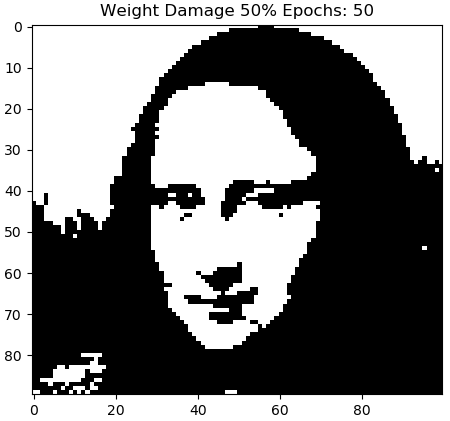
\includegraphics[scale=0.34]{images/mona_chn_50_end.png}
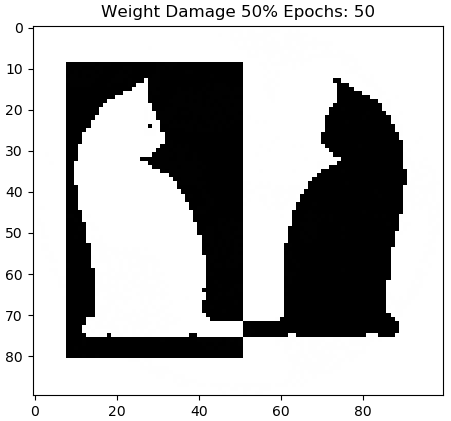
\includegraphics[scale=0.34]{images/cat_chn_50_end.png}
\caption{RMSE variation when trained using a Continuous Hopfield Network, with 50\% Weight Damage}
\end{figure}

\noi
\textbf{Image Retrieval Video}\\
The video of the image retrieval can be accessed in the files folder and are named: \tt{ball\_chn\_50.mp4}, \tt{mona\_chn\_50.mp4} and \tt{cat\_chn\_50.mp4}.


\subsubsection{80\% Weight damage}
\textbf{Variation of RMSE across Iterations}\\
The variation of RMSE across iterations using a continuous hopfield network is as follows:
\begin{figure}[H]
\centering
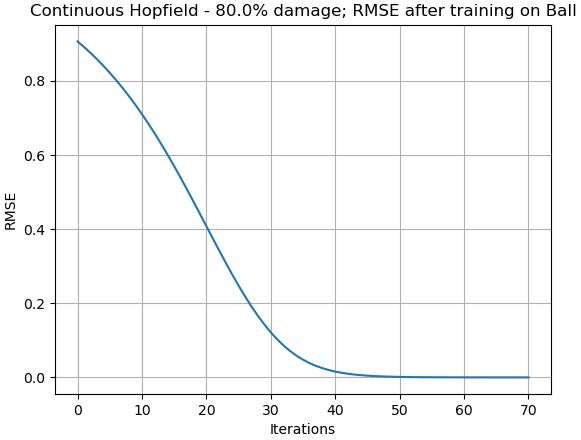
\includegraphics[scale=0.4]{images/chn_80_ball.png}
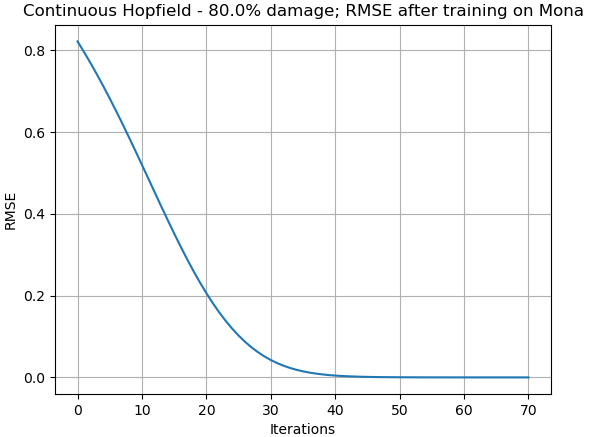
\includegraphics[scale=0.4]{images/chn_80_mona.png}
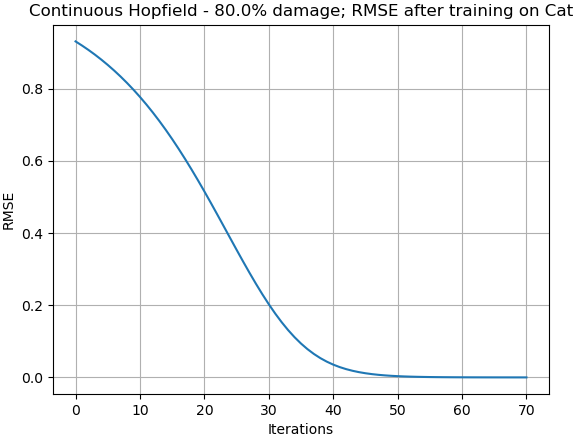
\includegraphics[scale=0.4]{images/chn_80_cat.png}
\caption{RMSE variation when trained using a Continuous Hopfield Network, with 80\% Weight Damage}
\end{figure}

\noi
\textbf{Final Image Reconstruction}\\
The final images reconstructed using continuous hopfield networks is as follows:
\begin{figure}[H]
\centering
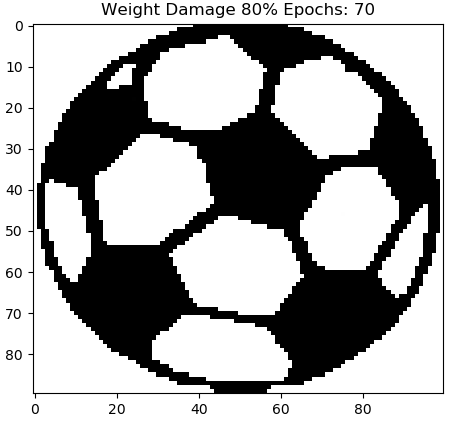
\includegraphics[scale=0.34]{images/ball_chn_80_end.png}
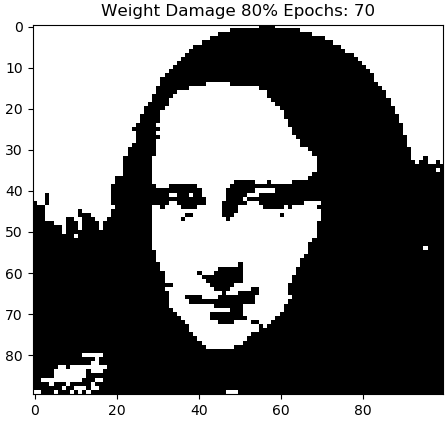
\includegraphics[scale=0.34]{images/mona_chn_80_end.png}
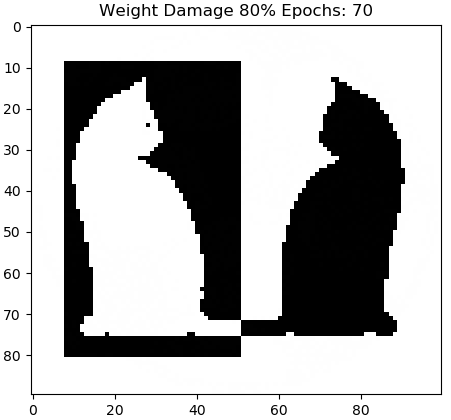
\includegraphics[scale=0.34]{images/cat_chn_80_end.png}
\caption{RMSE variation when trained using a Continuous Hopfield Network, with 80\% Weight Damage}
\end{figure}

\noi
\textbf{Image Retrieval Video}\\
The video of the image retrieval can be accessed in the files folder and are named: \tt{ball\_chn\_80.mp4}, \tt{mona\_chn\_80.mp4} and \tt{cat\_chn\_80.mp4}.


\end{document}
